\section{\textit{Helper application} como um chaveiro}
\label{chaveiro}

\quad Neste caso além da  \textit{helper application} implementar e expor as interfaces necessárias para permitir a execução correta e segura dos protocolos de autenticação com o IDP, este deve também implementar um serviço de chaveiro de credencias de \textit{login}, isto é, irá guardar localmente um conjunto de credenciais (username/email e \textit{passwords}) e o utilizador têm acesso a estes dados com um \textit{login} independente realizado na \textit{helper application} onde é protegido por uma chave mestra. Este serviço foi implementado para permitir a navegação do utilizador na interface gráfica (que é exposta pelo \textit{browser}), mas também permitir executar os processos de autenticação automaticamente, sem necessidade de interação do utilizador, isto é, imaginando que o utilizador já tem uma sessão iniciada localmente no chaveiro, caso este tente aceder ao serviço exposto pelo SP e não tenha sessão iniciada, o processo de autenticação com o uso do padrão SAML nas mensagens é feito automaticamente. 

\quad Portanto, neste caso o chaveiro protege um conjunto de credenciais que permite ao utilizador autenticar-se usando os serviços do IDP, ou seja, este serviço armazena uma lista de credenciais em que cada entrada está relacionada a um IDP, como é observável na figura \ref{fig:accounts}. Para garantir a privacidade e segurança das senhas das contas, estas são armazenadas localmente pela \textit{helper application} cifradas usando o algoritmo AES cujo segredo é a chave mestra do chaveiro.

\begin{figure}[H]
    \caption{Lista de contas de um utilizador por IDP (após o login com a chave mestra)}
    \label{fig:accounts}
    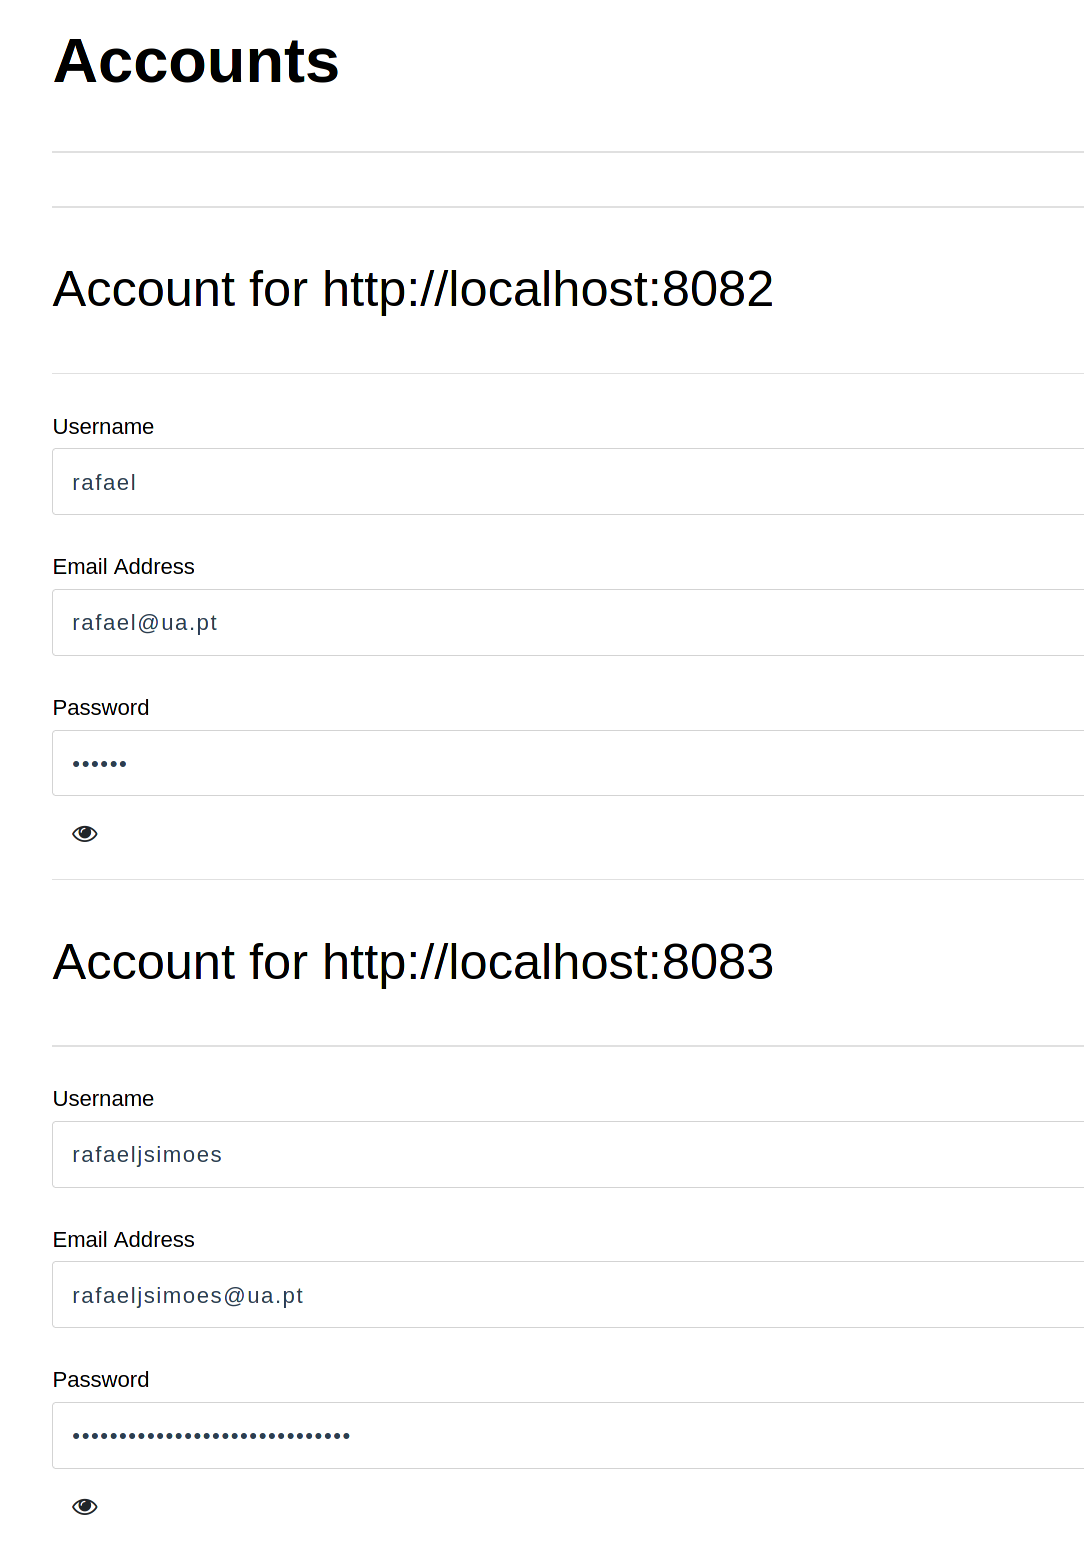
\includegraphics[width=0.7\textwidth, height=0.7\textheight]{img/accounts.png}
    \centering
\end{figure}

\quad Uma vez que o utilizador pode iniciar sessão com o serviço exposto pelo SP em diferentes dispositivos, o IDP tem de ter a capacidade de armazenar múltiplas chaves publicas uma por cada dispositivo diferente, ou seja, o mesmo utilizador pode ter vários pares de credenciais assimétricas para a mesma conta em dispositivos informáticos diferentes. Como é óbvio, a \textit{helper application} tem de ter a capacidade de poder gerir várias contas de chaveiro no mesmo dispositivo, permitindo múltiplas contas de utilizador localmente.


\quad Finalmente, como já foi referido anteriormente, uma vez que este chaveiro têm um sistema de \textit{login} independente, é importante criar sessões neste serviço para permitir o utilizador fazer a navegação livre na interface gráfica e para agilizar o processo de autenticação com o IDP, pois caso exista uma sessão ativa e válida com a \textit{helper application} o processo de autenticação com o IDP (começado pelo SP) é completamente automático, pois a aplicação tem a capacidade de mascarar todos os mecanismos necessários para inicializar tais processos, como:
\begin{itemize}
    \item Através do \textit{session id} enviado pelo \textit{browser} (que está armazenado nas \textit{cookies}), a \textit{helper application} obtém os dados necessários do utilizador. Neste caso é necessário o IDP enviar um identificador da sua entidade, para \textit{helper application} perceber quais da entradas da lista de credenciais este deve usar.
    \item Depois com os dados dos utilizadores e o identificador do IDP, a \textit{helper application} consegues retornar os dados das credenciais relativos à conta pretendida, e faz decifra (e verificação com o valor de MAC) da \textit{password} da conta para esta poder ser usada nos processo seguintes de autenticação.
\end{itemize}

\quad Para finalizar, é apenas importante de referir que caso o SP comece o processo de autenticação e o utilizador não tenha uma sessão iniciada com o serviço de chaveiro, a \textit{helper application} pede ao utilizador para fazer a autenticação local usando a chave mestra para poder criar uma sessão. De seguida, o processo de autenticação procede-se como relatado anteriormente \footnote{É necessário garantir que o utilizador tem uma conta para o IDP pretendido, caso contrário o chaveiro apresenta uma página para a adição de credenciais para um IDP, que além de guardar localmente estas credenciais, envia também os dados para o IDP para este poder persistir estas informações (explicado em \ref{chaveiro_extras}), contudo o processo de autenticação inicial com o IDP é interrompido}.

\subsection{Extras}
\label{chaveiro_extras}

\quad Apesar de no enunciado deste relatório afirmar que a gestão e criação de contas podia ser feita de forma manual com interação direta com o mecanismo de persistência (que neste caso é sqlite3), foram implementado duas \textit{features} extras.

\begin{itemize}
    \item Criação de contas de chaveiro na \textit{helper application} - \ref{fig:chaveiro_create_acc}.
    \item Adição de uma conta com as credencias para um IDP, este mecanismo além de armazenar os dados da conta localmente na \textit{helper application} envia os dados introduzidos para o IDP para permitir a adição destas credenciais no IDP, para que os processos de autenticação usando estas credenciais executem corretamente - \ref{fig:create_idp_account}.
\end{itemize}


\begin{figure}[H]
    \centering
    \subfloat[Criação de conta no chaveiro]{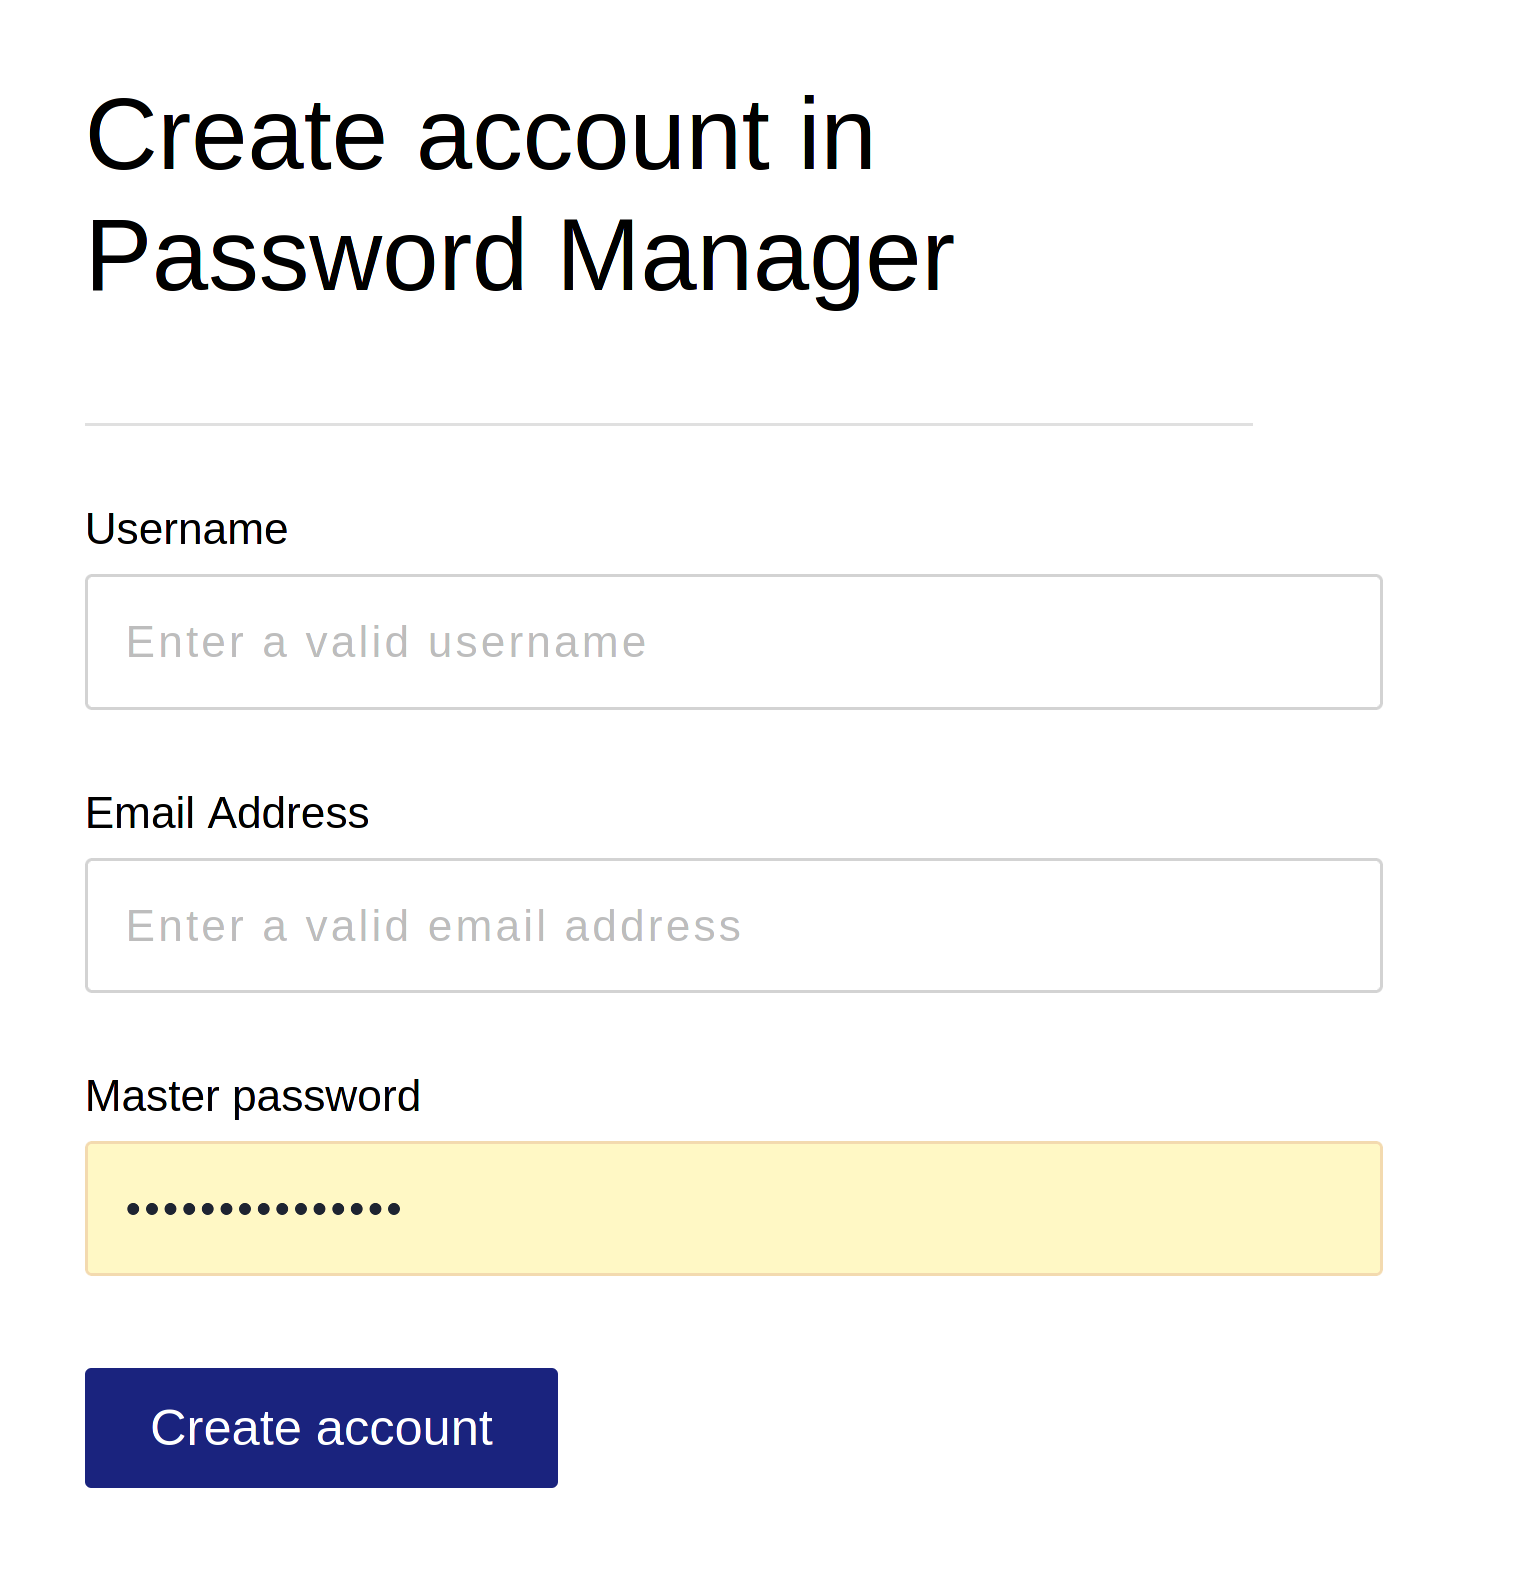
\includegraphics[width=0.3\textwidth]{img/chaveiro_create_acc.png}\label{fig:chaveiro_create_acc}}
    \hfill
    \subfloat[Criar conta num IDP]{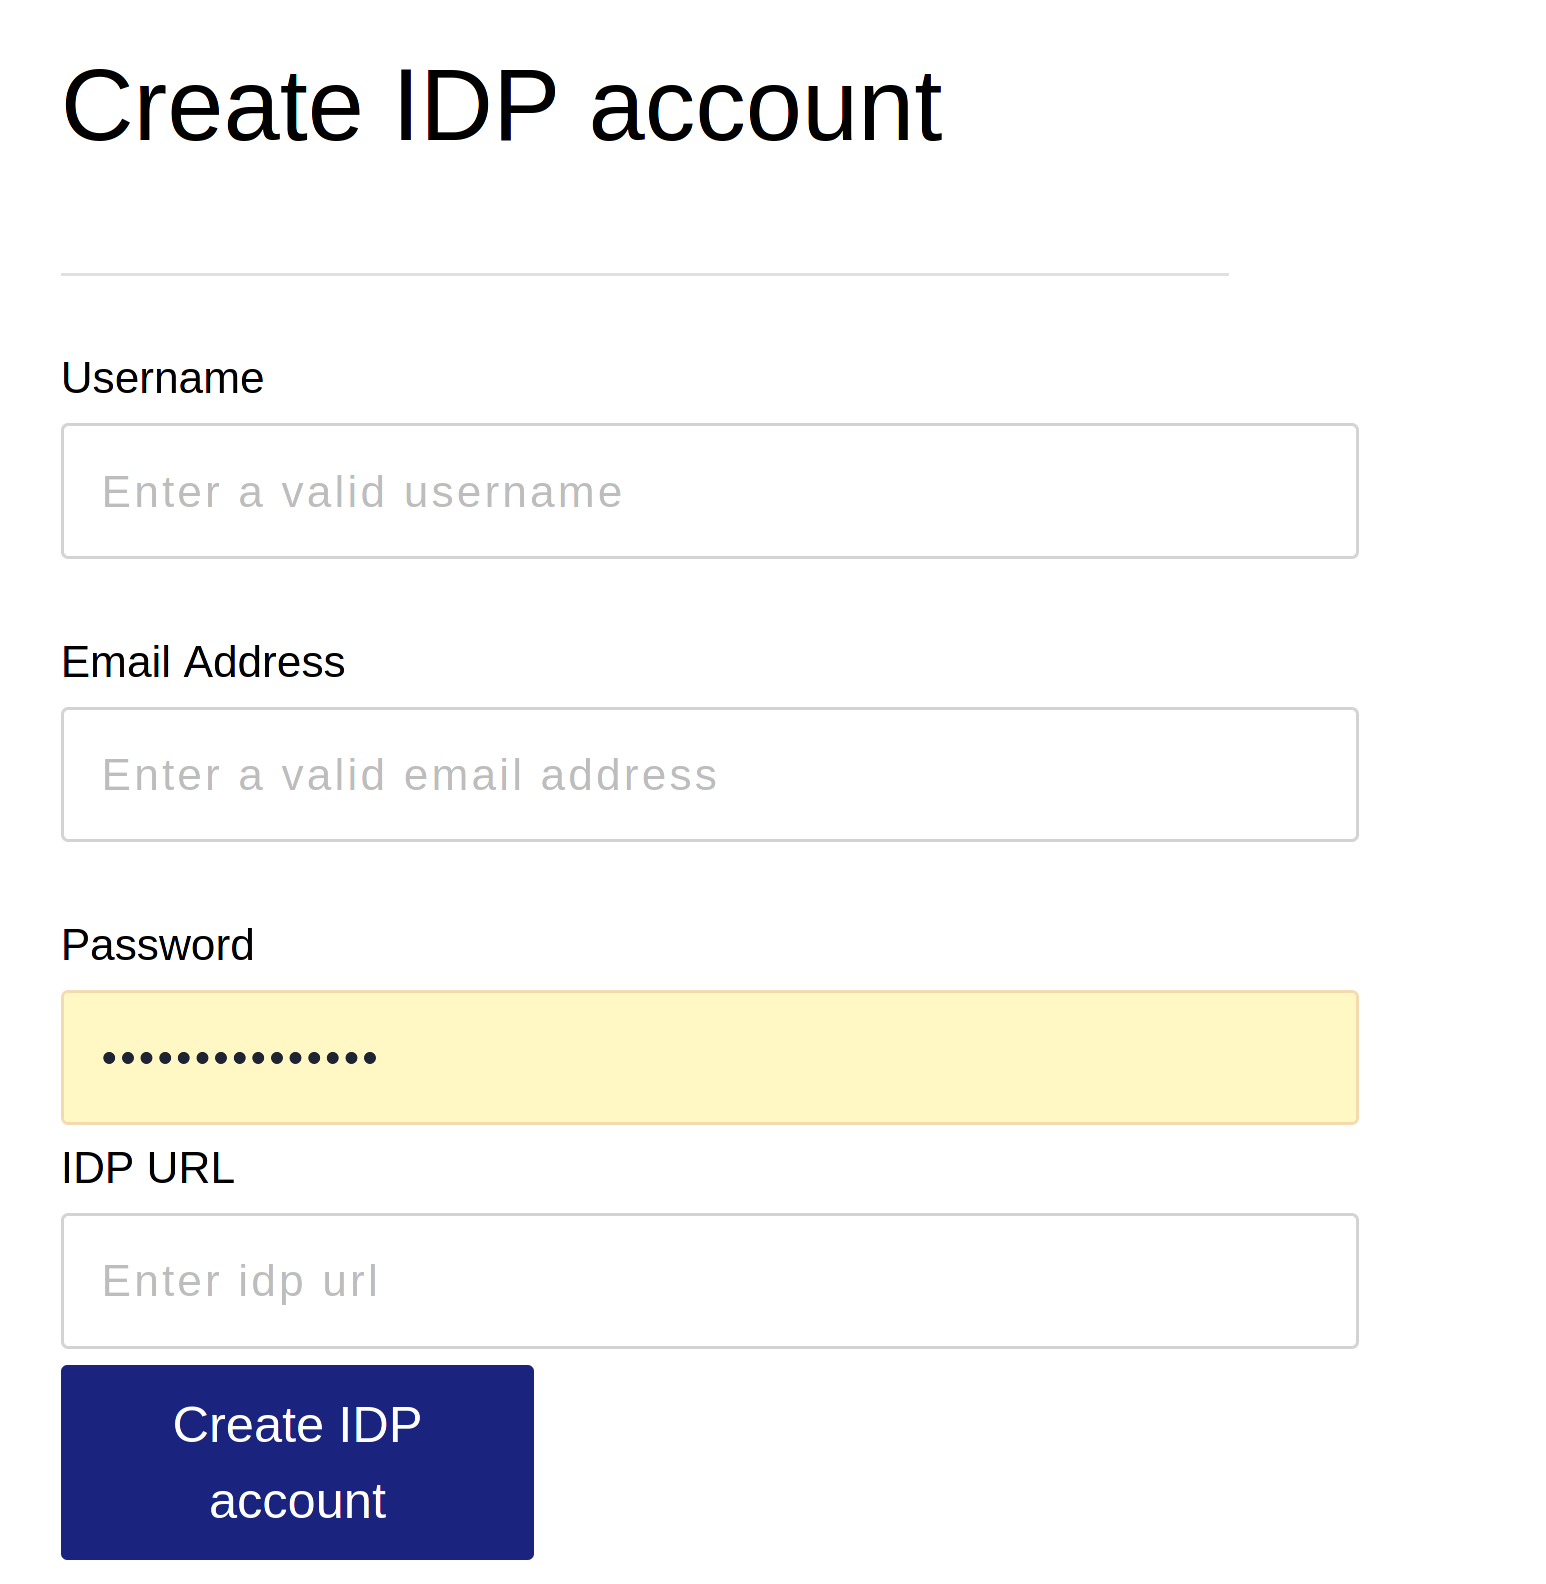
\includegraphics[width=0.3\textwidth]{img/create_idp_account.png}\label{fig:create_idp_account}}
\end{figure}